\documentclass[twoside]{report}
% \documentclass{report}
\usepackage[utf8]{inputenc}
\usepackage{graphicx}% Required for inserting images
%\usepackage{CormorantGaramond}
\usepackage{mathptmx}
\usepackage[a4paper,
            left=50mm,
            right=30mm,
            top=40mm,
            bottom=50mm,
            footskip=.25in]{geometry}
\usepackage{blindtext}
\usepackage{multicol}
\usepackage{datetime}
\usepackage{titlesec}
\usepackage{type1cm}
\usepackage{xparse}
\usepackage{expl3}
\usepackage{setspace}
\usepackage{lettrine}
\usepackage[
    bookmarks=true,
    bookmarksopen=true,
    bookmarksnumbered=true,
    bookmarksopenlevel=1,
    pdfpagelabels=true,
    colorlinks=true,
    linkcolor=red,
    urlcolor=magenta,
    anchorcolor=black,
    citecolor=cyan,
    filecolor=magenta,
    menucolor=red,
    plainpages=false,
    hypertexnames=true,
    linktocpage=true,
]{hyperref}

\usepackage{lastpage}
\usepackage{fancyhdr}
\usepackage{afterpage}
\usepackage{hyperref}
\usepackage[acronym]{glossaries}

\usepackage[version=4]{mhchem}

\graphicspath{ {figures/} }
\usepackage{array}

\usepackage[backend=bibtex]{biblatex}
\addbibresource{citations.bib}

\usepackage[T1]{fontenc}

% \usepackage{amsmath}
\usepackage{amsfonts}
\usepackage{mathtools}
\usepackage{listings}
\usepackage{xcolor}
% \usepackage{fontspec} this deosn't work and its fucking frustrating
\usepackage{color}
% \usepackage{mathalfa}

% \usepackage[grid]{eso-pic}
% \usepackage{kantlipsum}
%\usepackage{show frame}


%----------------------------------------------------------------------------------------%
% SETUP OF THE BACKEND


\titleformat{\chapter}{\normalfont\large\bfseries}{\thechapter $\hskip1em$ $\mid$}{1em}{}
\titlespacing*{\chapter}{10pt}{5mm}{3mm}

\titleformat{\section}{\normalfont\normalsize\bfseries}{\thesection}{1em}{}
\titlespacing*{\section}{20pt}{10mm}{3mm}

\titleformat{\subsection}{\normalfont\normalsize}{\thesubsection}{1em}{}
\titlespacing*{\subsection}{20pt}{10mm}{3mm}

% Set line spacing to 1.5
\setstretch{0.7}

\setlength\parindent{24pt}

\DeclareGraphicsExtensions{.pdf,.jpeg,.png}


% \pagenumbering{gobble} % Suppresses the page numbering
\pagestyle{fancy}
% Pied de page
\fancyfoot[L]{}
\fancyfoot[R]{}
\fancyfoot[C]{}
% \fancyfoot[C]{\it Page \thepage\ of \pageref{LastPage}}
% \fancyhead[ro, le]{\it Page \thepage\ of \pageref{LastPage}}
% \fancyhead[L]{}
% \fancyhead[R]{}
% \fancyhead[C]{}

\renewcommand{\headrulewidth}{0pt} % Deletes the horizontal line of the header
\newcommand{\innerp}[2]{\left\langle #1 #2 \right\rangle}
\newcommand{\proj}[2]{\left\langle #1 , #2 \right\rangle}

% Code snippet setup
\definecolor{codegreen}{rgb}{0,0.6,0}
\definecolor{codegray}{rgb}{0.5,0.5,0.5}
\definecolor{codepurple}{rgb}{0.58,0,0.82}
\definecolor{backcolour}{rgb}{0.95,0.95,0.92}

\lstset{
    basicstyle=\ttfamily\smallsize, 
    keywordstyle=\color{blue},
    commentstyle=\color{gray},
    stringstyle=\color{red},
    numbers=left,
    numberstyle=\tiny\color{gray},
    stepnumber=1,
    numbersep=10pt,
    backgroundcolor=\color{white},
    showspaces=false,
    showstringspaces=false,
    showtabs=false,
    frame=single,
    tabsize=4,
    captionpos=b,
    breaklines=true,
    breakatwhitespace=false,
    title=\lstname,
    escapeinside={(*@}{@*)}
}


%----------------------------------------------------------------------------------------%
% ACRONYMS

\makenoidxglossaries

\newacronym{OP1}{OP1}{Operation Phase 1}
\newacronym{OP2}{OP2}{Operation Phase 2}
\newacronym{W7-X}{W7-X}{Wendelstein 7-X}
\newacronym{PFCs}{PFCs}{Plasma Facing Components}
\newacronym{BCs}{BCs}{Boundary Conditions}
\newacronym{HS}{HS}{Heat Shield}
\newacronym{ECRH}{ECRH}{Electron Cyclotron Resonance Heating}


%----------------------------------------------------------------------------------------%
% SETUP OF THE DOCUMENT
\begin{document}
\begin{titlepage}
    \centering
    
\includegraphics[scale=0.075, angle=0]{figures/logo.jpg}\\
    \vskip2cm
    {\bfseries\normalsize
        \textsc{Institut National des Sciences Appliquées de Strasbourg}
        \\
    }
    {\small
        Department of mechanical engineering\\
    }
    {\bfseries\normalsize
        \textsc{Université de Strasbourg}
        \\
    }
    {\small
        Faculty of Physics and Engineering\\
    }
    \vskip3cm
    {\normalsize
        Master’s Thesis submitted in fulfillment of the requirements for the degrees of\\
        \it Master of Engineering\\
        \it Master of Science\\
    }
     \vskip1cm
    {\bfseries\huge
        Nonlinear thermal and structural finite element analysis of selected in-vessel components of W7-X\\
    }
    \vskip3cm
    \setlength{\columnsep}{0cm}
    \begin{multicols}{2}
        \begin{flushleft}
        {\it\small{Author:}}
        \\
        {\bfseries\large{Nicolas Olive-Leriche}}
        \\ 
        {\normalsize{Mechanical engineering/Applied physics and physical engineering}}
        \\
        \end{flushleft}
    \columnbreak
        \begin{flushright}
        {\it\small{Academic supervisor:}}
        \\
        {\bfseries\normalsize{MdC. \textsc{Mathieu Solar}}}
        \\ 
        {\normalsize{INSA Strasbourg}}
        \\
        {\normalsize{Institut Charles Sadron}}
        \vskip.25cm
        {\it\small{Professional tutor:}}
        \\
        {\bfseries\normalsize{\textsc{Mikhail Khokhlov}}}
        \\ 
        {\normalsize{Max Planck Institute for Plasma Physics}}
        \\
        \end{flushright}
    \end{multicols}
    \vskip1cm
    {\small
        Greifswald, \the\year\\
    }
\end{titlepage}

\pagenumbering{roman}
\fancyhead[ro, le]{\it Page \thepage}
\fancypagestyle{plain}{
\fancyhf{} % Efface les en-têtes et pieds de page actuels
\fancyfoot[ro, le]{}
\fancyhead[ro, le]{\it Page \thepage} % Ajoute le numéro de page à droite
\renewcommand{\headrulewidth}{0pt} % Supprime la ligne d'en-tête
}

\afterpage{\null\newpage}
\afterpage{\null\newpage}
\chapter*{Acknowledgement}
\newpage
\chapter*{Abstract}
\newpage
% \chapter*{Table of content}
\tableofcontents
\newpage
\listoffigures
\newpage

% [type=\acronymtype]
\printnoidxglossaries
\printacronyms

\newpage
\fancyhead[ro, le]{\it Page \thepage\ of \pageref{LastPage}}
\pagenumbering{arabic}
\fancypagestyle{plain}{
\fancyhf{} % Efface les en-têtes et pieds de page actuels
\fancyfoot[ro, le]{}
\fancyhead[ro, le]{\it Page \thepage\ of \pageref{LastPage}} % Ajoute le numéro de page à droite
\renewcommand{\headrulewidth}{0pt} % Supprime la ligne d'en-tête
}

% Chapter implementation
\chapter{INTRODUCTION}
\lettrine[lines=3, lhang=0.33, loversize=0.25]{N}{uclear} \normalsize{fusion has been the subject of many years of research and different experiments conducted at all scales. This craze is mainly due to the possibility of clean, renewable and safe nuclear power generation. This idea of generating electricity via the fusion of light atomic nuclei finds its roots in the early 1950s when physicists tried different ways of containing a plasma using different techniques, one of which is called magnetic confinement. To know why such devices are necessary, a look at the physics behind nuclear fusion could help. Fusing light atomic nuclei require them to come close enough for the strong nuclear force to overcome the electrostatic force pushing them apart. One way to approach one nucleus to the other close enough to surpass the so-called Coulomb barrier is to heat the atoms to high temperatures or accelerate those particles enough to attain such energies. At those energies, the fuel becomes a hot plasma and can no longer be contained in a classical confinement.}
\\
\break
\normalsize{\indent Plasma is the fourth state of matter, consisting of ionized gas where atoms lose electrons. This ionization results in a mixture of positively charged ions and free electrons, making plasma distinct from solids, liquids, and gases. Plasmas exhibit unique properties, including responsiveness to magnetic fields and the ability to conduct electricity. They are prevalent in phenomena like stars, lightning, and certain man-made technologies such as fluorescent lights and plasma TVs. The pursuit of effective confinement for fusion plasma introduces various challenges of a complex nature. Stability concerns arise from inherent plasma instabilities, contributing to disruptions and energy dissipation. The prudent management of heat generated by fusion reactions assumes paramount importance to mitigate potential damage to plasma facing components. The research for materials suitable for the plasma facing components with enhanced durability requires overcoming challenges associated with extreme conditions, including elevated temperatures, neutron bombardment, and erosion.}
\\
\break
\normalsize{\indent Magnetic confinement, a crucial aspect of fusion devices, necessitates intricate manipulation of magnetic fields to attain stability and sustain plasma confinement. Establishing an energy equilibrium, where input aligns with output, constitutes a foundational imperative for realizing ignition in fusion reactions. The control of turbulence and transport phenomena within the plasma is essential to preclude unwarranted particle and energy transport, optimizing overall performance. The delicate equilibrium governing plasma density and temperature, vital for sustained fusion reactions, necessitates meticulous control and stability. Addressing these intricacies assumes pivotal significance in advancing fusion research and realizing the potential of fusion energy as a scientifically viable and sustainable power source. Wendelstein 7-X (\acrshort{W7-X}) is an experimental Stellarator fusion device located at the Max Planck Institute for Plasma Physics (IPP) in Greifswald, Germany. The purpose of \acrshort{W7-X} is to investigate the feasibility of generating energy through nuclear fusion.}

\section{PROBLEM DEFINITION AND OBJECTIVES}
\normalsize{W7-X enters its enhanced operation phase called \acrshort{OP2}. This operation phase aims to improve confinement time and heating power. To achieve longer runs and attain steady state operation, many different plasma parameters such as the temperature, the density and the pressure need to be fully controlled and piloted precisely. To gain this control and understand more the complex plasma dynamics of the reactors, longer plasma discharges will take place and provide to the physicists the desired data. Because the plasma discharges are longer and the plasma heated at higher powers than in Operation Phase 1 \acrshort{OP1}, the components surrounding the plasma, especially the plasma facing components (\acrshort{PFCs}) will be exposed to higher heat flux for a longer period of time. This will lead to increased wear on the system components due to high heat fluxes and can lead to mechanical failure. To assess this risk of failure, the engineering analysis group of the Experimental Plasma Physics 5 department conducts many different numerical analysis campaigns to predict the behavior of the device under special load cases.}
\\
\break
\normalsize{\indent In order to set boundaries on the pulses of \acrshort{OP2} and validate the proper functioning of the various subsystems, the thermal analyses as well as the mechanical analyses of various in-vessel components both steady and unsteady is carried out by the engineers. After early calculations, it was shown that. It is necessary for the \acrshort{ECRH} TZM-reflector tile to accommodate for high steady state heat flux. Steady state is assumed for the analysis since the plasma impulse is considered of long duration and the thermal equilibrium of the reflector tile attained. It is crucial to properly design and dimension the tile in order to allow the new operational parameters. Based on the modified TZM-reflector tile, thermal and structural finite element analyses of different load cases and boundary conditions \acrshort{BCs} will be conducted to validate the new design. Following the results of these analyses, the engineers will be able to set operational boundaries if necessary or validate the design and proceed with the operation. The results will also allow to know the different maximum operational parameters such as maximum operation time. The reliability of the calculations will influence the decision made and thus needs to be estimated to avoid any significant error between the FE model and the real life behavior.}
\\
\break
\normalsize{\indent First, a literature research is carried out to understand the physics involved in those phenomenon such as the link between temperature and mechanical properties of materials or the physics of radiative heat transfer. The reading of documents assessing those issues also helps put into context this work and lie the basis upon which this Thesis is being lead. Because this is entirely simulation based, the proper functioning of the analyzed components will be proved by locating their performances within an operational space defined by the designers under various load cases and meshes. In addition to that, this work is separated into main tasks, the steady state as well as transient thermal and mechanical FEA of the \acrshort{ECRH} TZM-reflector tile. To do that, the modelling and setup of the different geometries as well as the clarification and characterization of the physics, material properties and \acrshort{BCs} and the analyses and discussions about the results will be necessary.}

\section{STRUCTURE OF THE THESIS}
\normalsize{In the first third section of the Thesis, the theoretical foundations for practical work are explained. These include the basics of nuclear fusion and fusion devices but also concepts of heat transfer and solid mechanics. This will help setting up a link between the two and allow building and propose a performance indicator based on positions in an operational space to validate proper functioning.}
\\
\break
\normalsize{\indent The second and the third sections, the methods and models as well as the results and the discussions of the analyses will be done and concluded at the very end of this work.}
\newpage
\chapter{THEORETICAL FRAMEWORK}
\normalsize{In this chapter, the basics of fusion such as nuclear physics and magnetic confinement are explained. In addition to that, the construction and the different systems of the W7-X are also explained to give an overview on the device and its auxiliary components. Heat transfer theory as well as solid mechanics including plasticity and fatigue constitute the basis of the work and the complex equations of these theories solved using Finite Element Analysis. These theories are necessary for the completion of this work and are therefore reminded in this chapter.}
\section{GENERAL THEORY OF FUSION REACTORS}
\normalsize{The principle of a nuclear fusion power plant is to make the energy released by the fusion of light atomic nuclei usable. Nuclear fusion which represent the fusing of atomic nuclei together is only achievable if they come close enough to surpass the electrostatic repulsion forces and have the strong nuclear force fuse the nucleons together. Due to electrostatic repulsion forces also called Coulomb barrier, the nuclei repulse each other thus preventing the reaching of the necessary distance (because the strong nuclear force has a very limited range, ~$10^{-15}$m) \cite{diekmann_energie:_2014}\cite{Freidberg_2007} for fusion. Furthermore, the repulsion forces increase with the number of protons in the nucleus or its size. The energy required to fuse two nuclei become subsequently greater.}
\\
\begin{figure}[h!] 
    \centering
    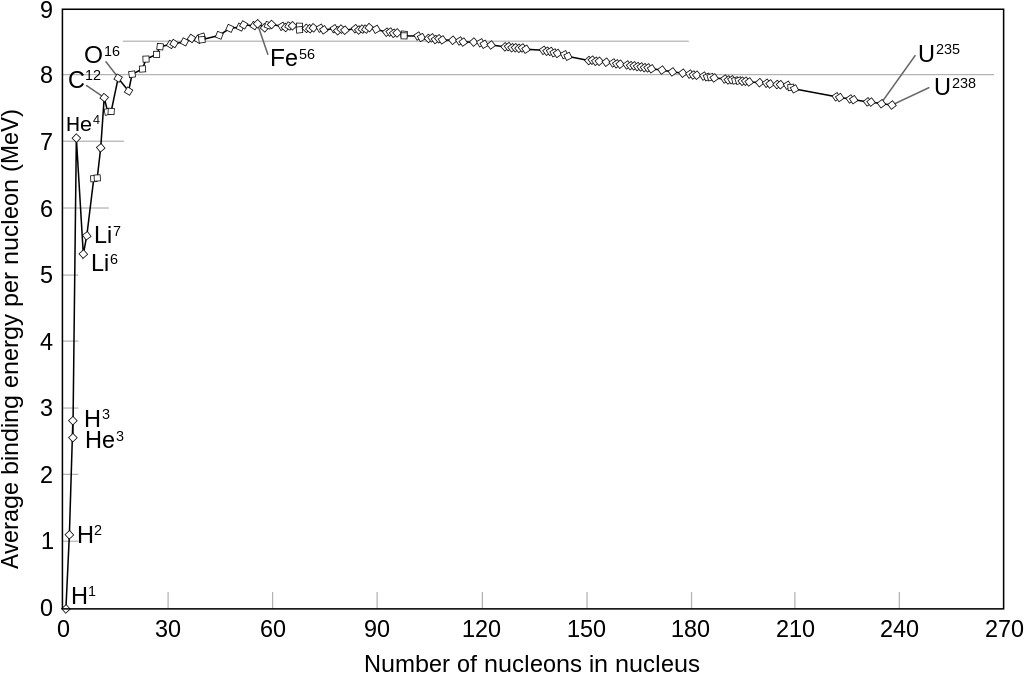
\includegraphics[width=.7\textwidth]{figures/fig_1.png}
    \caption{\it Nuclear binding energy vs. mass number.}
    \label{fig:fig_2_1}
\end{figure}
\\
\normalsize{\indent The different nuclear reactions for transforming hydrogen into helium are \cite{diekmann_energie:_2014}:}
\begin{equation}
    \ce{^1_1H + ^1_0n -> ^2_1H + 2.22 MeV\footnote{Automatically generated footnote markers work fine!}}
\end{equation}
\begin{equation}
    \ce{^2_1H + ^1_1p -> ^3_2He + 5.49 MeV}
\end{equation}
\normalsize{\indent or}
\begin{equation}
    \ce{^2_1H + ^2_1H -> ^3_2He + ^1_0n + 3.27 MeV}
\end{equation}
\begin{equation}
    \ce{^2_1H + ^2_1H -> ^3_1He + ^1_1p + 4.03 MeV}
\end{equation}
\begin{equation}
    \ce{^2_1H + ^3_1H -> ^4_2He + ^1_0n + 17.58 MeV}
\end{equation}
\\
\normalsize{\indent On Figure \ref{fig:fig_2_2}, the cross section for various reactions are graphed in function of the ion temperature. The cross section represents the area on which it is possible for nuclei to collide and subsequently fuse together. The higher the cross section, the higher the nuclei are likely to collide with each other. For lower ion temperatures, the Deuterium-Tritium reaction has the biggest cross section. The easiest way to initiate fusion is by the Deuterium–Tritium reaction, which releases $17.6 MeV$, $14.1 MeV$ in the neutron and $3.5 MeV$ in the alpha particle. \cite{Freidberg_2007}}
\\
\begin{figure}[h!]
    \centering
    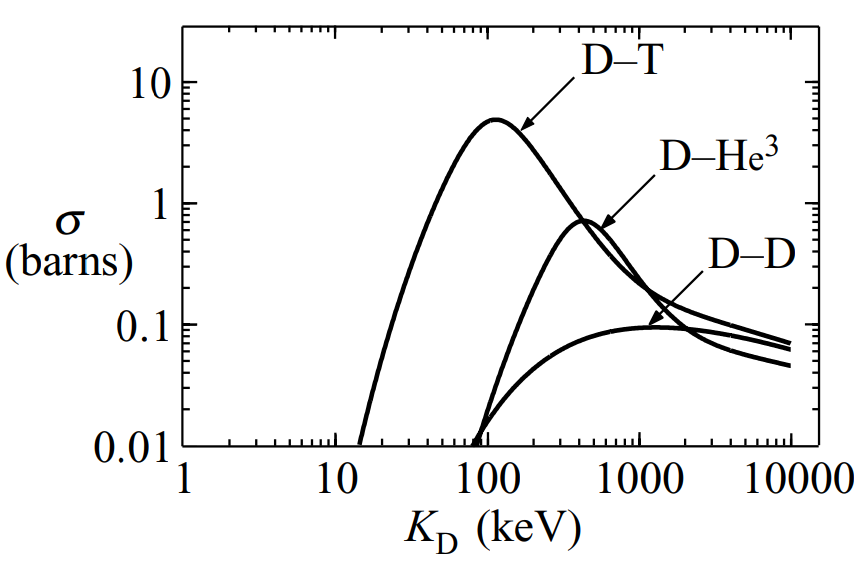
\includegraphics[width=.62\textwidth]{figures/crosssection.png}
    \caption{\it Fusion cross sections for various fusion reactions (D-T, D-$He^3$ and D-D) versus ion temperature. \cite{Freidberg_2007}}
    \label{fig:fig_2_2}
\end{figure}
\\
\normalsize{\indent When the cross section is known, is it possible to calculate the reaction rate for the main fusion reactions. The reaction rate is noted $\innerp{\sigma}{\nu}$. These results are illustrated in Figure \ref{fig:fig_2_3} as curves of $\innerp{\sigma}{\nu}$ vs. ion temperature $T$. It is possible to observe that the peak value of the reation rate is $9 \times 10^{-22} m^{3}s^{-1}$ at $70keV$ for the D-T fuel mix.}
\\
\begin{figure}[h!]
    \centering
    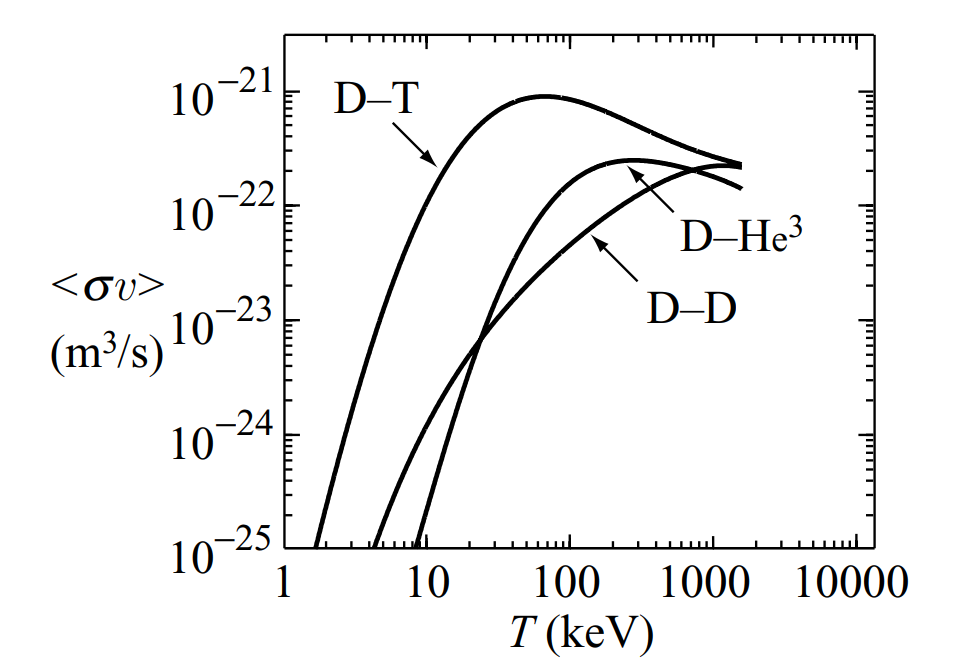
\includegraphics[width=.67\textwidth]{figures/reactionrate.png}
    \caption{\it Velocity averaged cross section $\innerp{\sigma}{\nu}$ for various fusion reactions (D-T, D-$He^3$ and D-D) versus ion temperature. \cite{Freidberg_2007}}
    \label{fig:fig_2_3}
\end{figure}
\\
\normalsize{\indent }
\\
\normalsize{\indent As said previously, the energies to achieve nuclear fusion are important. One solution to this problem is to give the correct amount of kinetic energy to the nuclei in order for them to overcome the Coulomb barrier. This kinetic energy is measured in Electron-Volts and is obtained by heating the fuel to high temperatures. The temperature thus reaches ~100M to 200M°C \cite{diekmann_energie:_2014}, which is hotter than the sun’s core. At those temperatures, the fuel becomes a plasma, which is often considered as the fourth state of matter. Plasma is also called the highest state of aggregation of a substance designated. In this aggregate state, the internal energy is far higher than the binding energy between the electrons and the nuclei. This means that the electrons can move freely. Plasma differs greatly in its properties from normal gases.}
\\
\break
\normalsize{\indent The important temperature of the plasma forces various measures to be taken to ensure that the Materials built into the fusion reactor near the plasma provide maintained thermal insulation and compensate for the resulting expansion pressure. A solution to this problem is the exploiting of the Lorenz force affecting the charged particles of the plasma. The idea is, at least for magnetic confinement, to trap the plasma inside a magnetic cage. This will help levitating the plasma and control its shape and position to avoid touching any \acrshort{PFCs}. The distance between the plasma and the \acrshort{PFCs} is crucial since contact could generate plasma turbulence or contaminate the plasma with impurities, reducing the quality of it. Different systems where developed to build such a confinement. }
\\
\break
\normalsize{\indent There are two different type of magnetic confinement concepts that are widely know and developed, the Tokamak and the Stellarator. These two magnetic confinement devices are both based on a toroidal geometry, the difference between the two of them being the way the plasma is confined. In a Tokamak machine, the plasma is confined using planar toroidal magnetic coils. Those coils help create the toroidal magnetic field component of the confinement. Although this seems like a good confinement, other problems still need to be addresses such as the effect of particle drift. This drift is due to  pressure gradients and inhomogeneities in the magnetic field inside the plasma and leads to a drift of the particles towards the outer diameter of the Tokamak. This complex particle transport phenomenon can be mitigated by introducing a poloidal component to the magnetic field, causing a rotation of the plasma around its toroidal axis. To achieve this magnetic field, Tokamaks use a solenoid coil placed at the center of the torus. This solenoid coil acts as a primary transformer coil, a time-varying electric current generate a varying magnetic field which itself induce an electric current inside the plasma. The resulting movement of charges inside the plasma generate a poloidal magnetic field, the plasma is then generating its own magnetic field. This electric current can also be used to heat up the plasma, it is called ohmic heating.}
\break
\begin{figure}[h!]
    \centering
    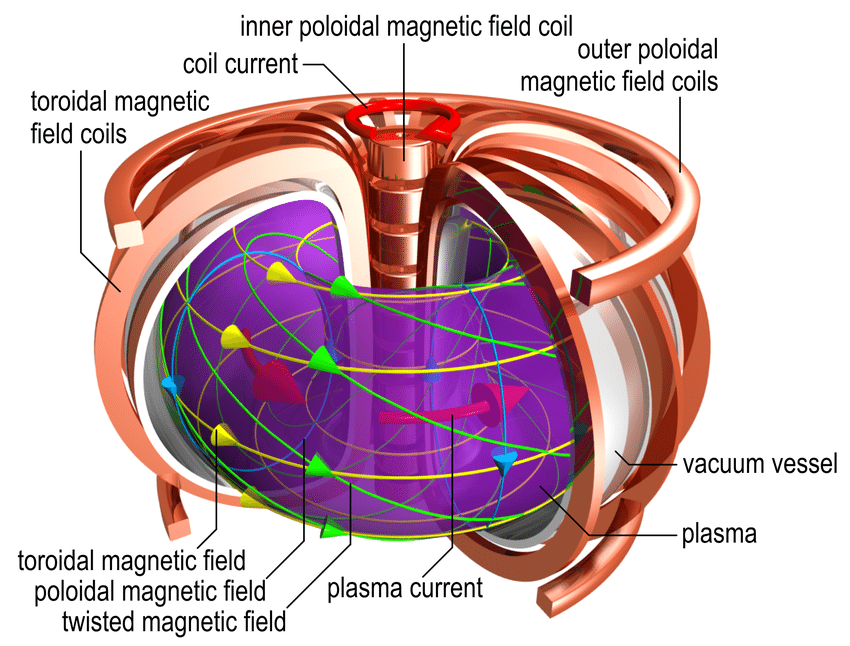
\includegraphics[width=.6\textwidth]{figures/fig_2.png}
    \caption{\it Schematics of a Tokamak confinement, courtesy of C. Brandt}
\end{figure}
\\
\break
\normalsize{\indent While this solution is good, there are problems with it. The main issue is the inherently transient process. The poloidal component of the magnetic field can only be generated as long as the current in the solenoid coil varies. This means that the reactor can only run in pulses and steady-state isn’t currently achievable.}
\\
\break
\normalsize{\indent Another solution for generating the poloidal magnetic field is to twirl the plasma in such a shape, that the drift phenomenon disappears. This solution is the Stellarator. The Stellarator was first introduced by Lyman Spitzer in the 1950s. This technology was put aside because of technical difficulties and because the Tokamaks presented better performances. The Stellarators use a complex set of magnets allowing to generate a precise magnetic field allowing the plasma to not experience significant drift. Contrary to Tokamaks, Stellerators plasmas don’t have a plasma current. This solution also helps with confinement, as the magnetic field can be adjusted to accommodate for the strict equilibrium conditions. The absence of plasma current also means that Stellarators can be operated in steady-state since no current induction is needed, thus being more suitable for power plants. Although allowing improved plasma confinement, Stellarators are plagued by complex geometries that are often too complex to be feasible.}
\begin{figure}[h!]
    \centering
    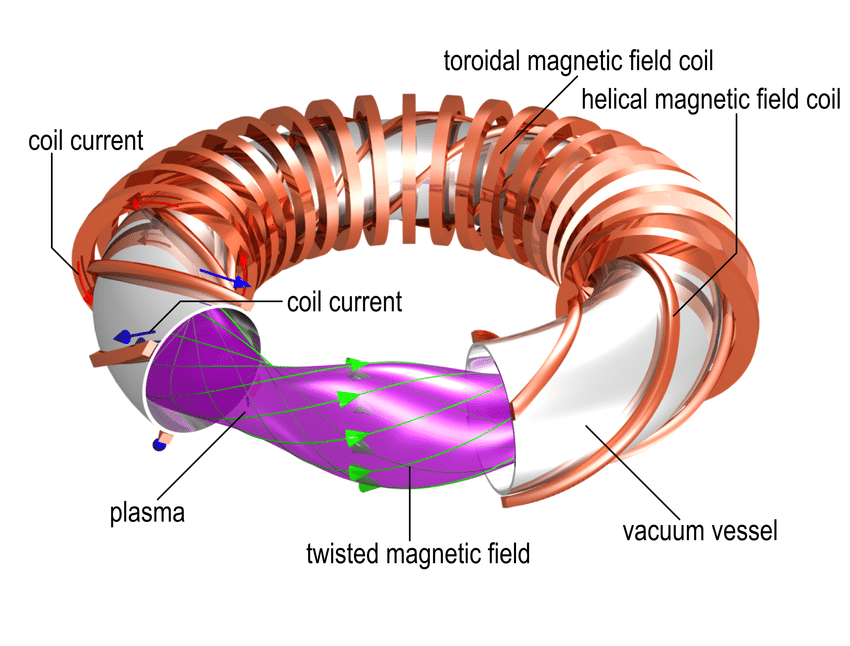
\includegraphics[width=.6\textwidth]{figures/fig_3.png}
    \caption{\it Schematics of a Stellarator confinement, courtesy of C. Brandt}
\end{figure}
\\
\normalsize{\indent The goal of those magnetic confinement fusion reactors concepts is to propose a new way of producing atomic energy while avoiding the drawbacks of traditional fission reactors (ie. Management of radiation, production of highly radioactive long half-life elements, limited fuel supply…). Although fusion energy is attractive, many problems still need to be addresses such as tritium breeding issues or neutron transport and interaction with the structure.}
\section{W7-X SYSTEMS}

\section{HEAT TRANSFER}
\normalsize{In this section, the fundamental principles and governing equations and each heat transfer mode are explored. The TZM-reflector tile is a highly constrained mechanical part that of the \acrshort{HS}. This part will be exposed to plasma radiation as well as the \acrshort{ECRH} beam.}




\section{SOLID MECHANICS}

\section{FINITE ELEMENT METHOD}


\newpage
\chapter{STATE OF THE ART}
\newpage
\chapter{METHODS AND CONFIGURATIONS}
\normalsize{As stated in the state of the art; the object of these analyses is the \acrshort{ECRH} TZM-reflector tile (ref. E821). To study the thermal and mechanical behavior of this in-vessel component, finite element analysis using the ANSYS\textsuperscript{\textregistered} software will be carried out to evaluate the new design's performances and the proposed solution to the overheating of the CuCrZr heat sink issue. Coupled physics analyses, in particular one-way coupling and full coupling of thermal and structural analyses, will be used to assess the effects of the design changes and validate the proper functioning of the reflector tile in \acrshort{OP2} design loads.}

\section{MATERIAL PROPERTIES AND PHYSICAL MODELS}
\section{CONTACT CONFIGURATION}
\section{PLASMA HEAT LOAD}
\section{MODELLING OF THE ECRH BEAM}
\subsection{Calculation of the integration coefficients}
\normalsize{The issue was in the parameters of the \acrshort{ECRH} beam load distribution since it was not clearly defined in the recalculation task requested by Torsten Stange. The little information about the parameters of the beam load were the nominal total heat flow of 912W, Gaussian shape of power distribution and the geometric properties of both axisymmetric and non-axisymmetric distribution. Based on these data, a series of calculations aiming to recalculate the load distribution on the tile surface  were undergone and provided good results.}
\begin{figure}[h!]
    \label{fig_4_1} 
    \centering
    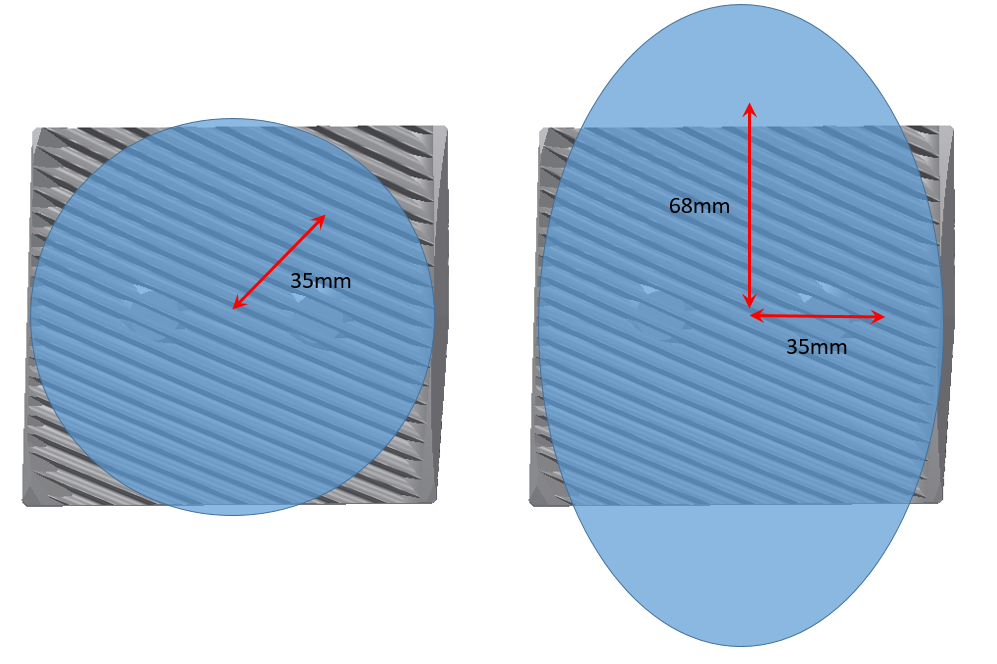
\includegraphics[width=.9\textwidth]{figures/TWOBEAMDISTRI.png}
    \caption{\it Representation of the two ECRH beam heat flux distribution cases}
\end{figure}
\\
\normalsize{\indent The calculation of the integral parameters as well as the analytical calculation of the surface integrals were done on Wolfram Mathematica\textsuperscript{\textregistered}. There are two different cases, one axisymmetric (circular) and another non-axisymmetric (elliptical). For the first case, almost all of the power ~99\% hits the ECRH reflector tile. The standard deviation is defined to be 35mm, for debug and validation purposes, 86\% of the power should be included within a disk of radius 35mm. For the elliptical distribution, much less power hits the reflector tile. The distribution properties are also different and feature two different radii, the minor semi-radius and the major semi-radius. Their values are respectively 35mm and 68mm, both of them defining an ellipse. Similarly to the circular distribution, for debugging, 86\% of the overall power should be included within the area of the ellipse.}
\\
\break
\normalsize{\indent With help of those information, the integration coefficients could be calculated. The first integral was expressed in a cylindrical coordinate system. The first APDL code written by J. Zhu \cite{zhu_parametric_2019} in 2019 only featured the circular heat flux distribution and was based on calculations made by Torsten Stange. The integrated function for Gaussian distribution has the form $\exp(-2r^2)$. The surface integral can be written:}
\\
\begin{equation}
    \int\displaylimits_{\Omega} \exp(-2r^2) \ dS \
\end{equation}
\\
\normalsize{in cylindrical coordinates, \it{$dS = rdrd\theta$}}
\normalsize{and $\Omega$ a surface in $\mathbb{R}^2$. When taking the normal distribution, is it possible to rewrite the function and include the standard deviation $r_0$. The integral $\mathbb{I}$ of $f$ on $\Omega$ is:}
\\
\begin{equation}
    \mathbb{I}_{\Omega}^f = \int\displaylimits_{\Omega} \exp\left(-2\left(\frac{r}{r_0}\right)^2 \right) \,dS
    \label{eqn:4.2}
\end{equation}
\\
\normalsize{When developing the differential (in cartesian coordinates), the integral becomes:}
\\
\begin{equation}
    \int\displaylimits_{\Omega} \exp\left(-2\left(\frac{r}{r_0}\right)^2 \right) \,dS = \int\displaylimits_0^{+ \infty} \int\displaylimits_0^{2 \pi} \exp\left(-2\left(\frac{r}{r_0}\right)^2 \right) \,rdrd\theta
\end{equation}
\\
\begin{equation}
    \int\displaylimits_0^{+ \infty} \int\displaylimits_0^{2 \pi} \exp\left(-2\left(\frac{r}{r_0}\right)^2 \right) \,rdrd\theta = \int\displaylimits_0^{+\infty} \exp\left(-2\left(\frac{r}{r_0}\right)^2 \right) \ rdr \int\displaylimits_0^{2 \pi} \ d \theta
\end{equation}
\\
\begin{equation}
    = 2 \pi \int\displaylimits_0^{+\infty} \exp\left(-2\left(\frac{r}{r_0}\right)^2 \right) \ rdr
\end{equation}
\\
\normalsize{When calculated, the value of this integral is:}
\\
\begin{equation}
    2 \pi \int\displaylimits_0^{+\infty} \exp\left(-2\left(\frac{r}{r_0}\right)^2 \right) \ rdr = 6,125 \cdot 10^{-4} \pi
\end{equation}
\\
\normalsize{\indent This function is then normalized by multiplying both side by a coefficient $k_{norm}$ such as $k_{norm} \cdot 6,125 \cdot 10^{-4} \pi = 1$ This coefficient has a value of $519,69 \ m^{-2}$. Since heat flux is in $[Wm^{-2}]$, $k_{norm}$ needs to be in $[m^{-2}]$.  To validate the normalization, it is possible to integrate the same function, but only for the radius between 0 and standard deviation and multiplying the function by $k_{norm}$. This gives:}
\\
\begin{equation}
    k_{norm} \left[ \int\displaylimits_0^{r_0} \int\displaylimits_0^{2 \pi} \exp\left(-2\left(\frac{r}{r_0}\right)^2 \right) \,rdrd\theta \right] = 0,8646
\end{equation}
\\
\normalsize{\indent The integral power of the ECRH beam is 912 W. This means that normalized ECRH beam power distribution can be multiplied by the integral power. It is thus possible to define $q_0 \coloneqq P_{ECRH}^{beam} \cdot k_{norm}$. In the case of the circular ECRH Gaussian heat flux distribution, the value of $q_0=473957 \ Wm^{-2}$, this value will be used in the APDL code. The implemented function is, in cylindrical coordinates \eqref{eqn:cylCSGHD}:}
\\
\begin{equation}
    f_{axisym.}^{cyl. CS}(r) = P_{ECRH}^{beam} k_{norm} \exp\left(-2\left(\frac{r}{r_0}\right)^2 \right) [W/m^2]
\end{equation}
\\ 
\begin{equation}
    \color{red}\boxed{\color{black} f_{axisym.}^{cyl. CS}(r) = 473957 \exp\left(-2\left(\frac{r}{35[mm]}\right)^2 \right) [W/m^2]}
    \label{eqn:cylCSGHD}
\end{equation}
\\
\normalsize{\indent For the cartesian coordinates, the method of normalization is analog to the method used for the integral normalization in cylindrical coordinates. The choice of the cartesian coordinate system is because of the function for the elliptical \acrshort{ECRH} power distribution case and the way the ellipse is defined. Although it is possible to vary the radius in function of the angle while working in cylindrical coordinates, or use the ellipse equation and application of Fubini’s theorem in cartesian coordinates, another more practical approach was used to compute the integral. The function $f$ written in cartesian coordinates is as follows ($a$ is the minor semi-radius and $b$ is the major semi-radius):}
\\ 
\begin{equation}
    f(x,y) = \exp\left(-2\left(\left(\frac{x}{a}\right)^2 + \left(\frac{y}{b}\right)^2 \right) \right)
    \label{eqn:carCSGDnn}
\end{equation}
\\
\normalsize{The integral of the function over $\Omega$ is written:}
\\ 
\begin{equation}
    \mathbb{I}_{\Omega}^f = \int\displaylimits_{\Omega} \exp\left(-2\left(\left(\frac{x}{a}\right)^2 + \left(\frac{y}{b}\right)^2 \right) \right) \ dS
\end{equation}
\\
\normalsize{in cartesian coordinates, \it{$dS = dxdy$}}
\normalsize{and $\Omega$ a surface in $\mathbb{R}^2$. For the moment, the function \eqref{eqn:carCSGDnn} is integrated over $\mathbb{R}^2$. To normalize the integral, it is possible to proceed the same way than for the cylindrical integral \eqref{eqn:4.2}. }
\\
\begin{equation}
    \int\displaylimits_{\mathbb{R}^2} \exp\left(-2\left(\left(\frac{x}{a}\right)^2 + \left(\frac{y}{b}\right)^2 \right) \right) \ dS = \int\displaylimits_{- \infty}^{+ \infty} \int\displaylimits_{- \infty}^{+ \infty} \exp\left(-2\left(\left(\frac{x}{a}\right)^2 + \left(\frac{y}{b}\right)^2 \right) \right) \ dxdy
\end{equation}
\\
\normalsize{\indent If $a$ and $b$ are equal, the distribution is circular. The normalization coefficient for the cartesian should therefore be the same as the cylindrical one since the standard deviation of the distribution is the same, the function is just expressed in a cartesian coordinate system. Let $a = b = 35mm$, the integral becomes:}
\\
\begin{equation}
    \int\displaylimits_{- \infty}^{+ \infty} \int\displaylimits_{- \infty}^{+ \infty} \exp\left(-2\left(\frac{x+y}{35[mm]}\right)^2\right) \ dxdy = 6,125 \cdot 10^{-4} \pi
\end{equation}
\\
\normalsize{\indent The normalization coefficient is $519,69 \ m^{-2}$ and the integration coefficient $q_0=473957 \ Wm^{-2}$. This coefficient is the same as the one for the distribution expressed a cylindrical coordinates. To validate this, it possible to proceed the same as with the cylindrical distribution, integrating over a disk of radius $35 \ mm$. There is a problem with integrating the function on a circle in Cartesian coordinates, because the surface is a square of a rectangle. It is however possible to find an alternative solution to this problem using the Heaviside step function. The 2D-Heaviside step function is a discontinuous function defined as follows:}
\\
\begin{equation}
     \ H_{\Omega}(x,y) =
    \begin{cases}
        1 & \text{if } (x,y) \in \Omega\\
        0 & \text{if } (x,y) \in \mathbb{R}\setminus\Omega
    \end{cases}
    \label{eqn:HSF}
\end{equation}
\\
\normalsize{\indent The idea to calculate the integral over a circle or an ellipse is to multiply the integrated function by the Heaviside function \eqref{eqn:HSF} to project its values over a non-zero area defined by $\partial \Omega$, the closed perimeter of the surface.}
\\
\break
\normalsize{\indent The domain on which it is necessary to integrate is bounded by the circle equation $x^2 + y^2 = r_0^2$. Because the domain is a disk, the equation becomes $x^2 + y^2 \leq r_0^2$. The domain of the circle is thus $\Omega = \{ (x,y) \in \mathbb{R}^2, r_0 \in \mathbb{R} : r_0^2 - x^2 - y^2 \leq 0 \}$ and by the way the Heaviside step function \eqref{eqn:HSF} is defined in Wolfram Mathematica\textsuperscript{\textregistered}, it becomes $H(r_0^2 - x^2 - y^2)$.}
\\
\begin{figure}[h!] 
    \centering
    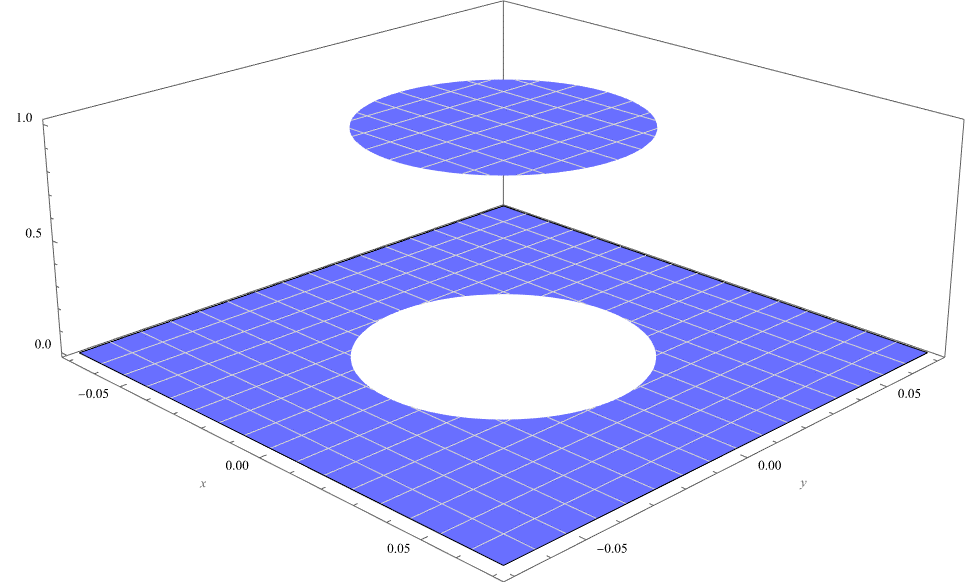
\includegraphics[width=.7\textwidth]{figures/stepfunction.png}
    \caption{\it 3D graph of the Heaviside step function defined over $\Omega$}
    \label{fig:fig_4_2}
\end{figure}
\\
\normalsize{\indent To validate the coefficient $k=519,69 \ m^{-2}$, it is possible to now integrate in Cartesian coordinates but on a disk. As said previously, the idea is to project the values of a function $f$ on a non-zero area $\Omega$ defined by $H_\Omega$, this is written as follows:}
\\
\begin{equation}
    \int\displaylimits_{\Omega_{cyl}} f \ rdrd\theta = \int\displaylimits_{\Omega_{car}} \proj{f}{H_\Omega} \ dxdy
\end{equation}
\\
\normalsize{with $\Omega_{cyl}$ being the cylindrical integration limits and $\Omega_{cyl}$ the cartesian integration limits. The fully written and calculated integral is :}
\\
\begin{equation}
    k \int\displaylimits_{-a}^{a} \int\displaylimits_{-b}^{b} \proj{\exp\left(-2\left(\frac{x+y}{35[mm]}\right)^2 \right)}{H(35[mm]^2 - x^2 - y^2 )} \ dxdy = 0,867
\end{equation}
\\
\normalsize{\indent The value of the integral is correct, and the integration coefficient for the Cartesian coordinates heat flux distribution is $q_0=473957 \ Wm^{-2}$,  which is the same as the cylindrical one. This is a good sight since the distribution are defined to be the same, it is reassuring to get the same result. For the elliptical one, the method is the same as the circular one except the argument in the Heaviside step function \eqref{eqn:HSF} isn’t derived for the circle equation but from the ellipse equation. The function for axisymmetric heat flux distribution written in cartesian coordinates is \eqref{eqn:carCSGHD}:}
\\
\begin{equation}
    \color{red}\boxed{\color{black} f_{axisym.}^{car. CS}(x,y) = 473957 \exp\left(-2\left(\frac{x+y}{35[mm]}\right)^2 \right) [W/m^2]}
    \label{eqn:carCSGHD}
\end{equation}
\\
\normalsize{\indent For the calculation of the non-axisymmetric integration coefficient (semi-minor radius of $35 \ mm$ and semi-major radius of $68 \ mm$), it is possible to proceed the same way as above. The ellipse is defined via the ellipse equation $(\frac{x}{a})^2 + (\frac{y}{b})^2 = 1$ with $a$ and $b$ being respectively the minor semi-radius and major semi-radius. The Heaviside step function \eqref{eqn:HSF} is written $H\left(1 - \left(\frac{x}{a}\right)^2 - \left(\frac{y}{b}\right)^2 \right)$. The normalization of the integral as well as the calculation of the integral on the ellipse is done the same way as before. The function on which the distribution $f$ is projected is the Heaviside step function \eqref{eqn:HSF} defined on an ellipse. The projection $\proj{f}{H_{\Omega}}$ is integrated and the results yields a normalization coefficient $k_{norm}$ of $267,5 \ m^{-2}$ and an integration coefficient $q_0$ of $243948 \ W/m^{2}$. The function for non-axisymmetric heat flux distribution written in cartesian coordinates is \eqref{eqn:carCSGHDNA}:}
\\
\begin{equation}
    \color{red}\boxed{\color{black} f_{non-axisym.}^{car. CS}(x,y) = 243948 \exp\left(-2\left(\left(\frac{x}{35[mm]}\right)^2 + \left(\frac{y}{68[mm]}\right)^2 \right) \right) [W/m^2]}
    \label{eqn:carCSGHDNA}
\end{equation}
\\
\normalsize{\indent All integration coefficients as well as the standard deviations of the distributions are summarized below:}

% INSERT THE SUMMARY TABLE

\subsection{Calculation of the surface integrales}


% Generate bibliography
\printbibliography

\end{document}
